\subsection{vagc}

Vagc is a simple graphics card which supports an 80x25 text mode with 16 colors and an RGB8 mode. 

\subsubsection{Text Mode}

The Text Mode allows to display 2000 characters. To do this vagc has an internal buffer of 4000 bytes. Each character 
to display requires two bytes. The first byte holds the information about foreground and background color and the second byte
is the actual character to be displayed. The buffer contains 25 rows of size 160. The position of a character in the
internal buffer is therefore defined as $2 * ((y * 80) + x)$. The character set used by vagc is standard ASCII for characters 33 to 126. However it
extends this character set with custom international characters. The graphic below shows all characters from 0 - 255 (0 is NW corner, 255 is SE corner, left to right). 
The higher nibble of the color information byte is the background color and the lower nibble of the color information byte is the foreground color (e.g. $0D41_{16}$ is a capital 'A' in white on black) (see~\elref{sec:colortable}). 

\begin{figure}[H]
\begin{center}
	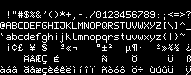
\includegraphics{./files/font.png}
\end{center}
	\caption{vagc font}
\end{figure}

\subsubsection{Color table}
\label{sec:colortable}

Given below is the color table for text mode:

\begin{tabular}{| r | r |}
	\hline
	$0_{16}$ & Black \\
	\hline
	$1_{16}$ & Red \\
	\hline
	$2_{16}$ & Green \\
	\hline
	$3_{16}$ & Blue \\
	\hline
	$4_{16}$ & Yellow \\
	\hline
	$5_{16}$ & Magenta \\
	\hline
	$6_{16}$ & Cyan \\
	\hline
	$7_{16}$ & Dark red \\
	\hline
	$8_{16}$ & Dark green \\
	\hline
	$9_{16}$ & Dark blue \\
	\hline
	$A_{16}$ & Dark yellow \\
	\hline
	$B_{16}$ & Dark magenta \\
	\hline
	$C_{16}$ & Dark cyan \\
	\hline
	$D_{16}$ & White \\
	\hline
	$E_{16}$ & Gray \\
	\hline
	$F_{16}$ & Dark gray \\
	\hline
\end{tabular}

\subsubsection{RGB Mode}

The RGB ode allows to display $480 \cdot 300 = 144000$ pixels. The internal RGB buffer is 144000 bytes in size. Each pixel is encoded in RGB8 format (3 bits red, 3 bits green, 2 bits blue). The position of a pixel in the internal buffer is defined as $(y * 480) + x$. 

\subsubsection{Writing to the vagc buffer}

There's no direct access to the internal vagc buffer. Vagc will issue a DMA read request of 4000 bytes (or 144000 in RGB mode) to a specified address. The address must be specified by writing to the vagc port which is port 16. Every write to the vagc port will issue a DMA read to the address that was written to port 16 and update the display.
Before writing again to the vagc port to update the internal buffer you must wait for hardware interrupt 16. 

\subsubsection{Switching modes}

To switch modes you have to tell vagc that the next write to its port is a command and not an address. Writing the invalid address $00000000_{16}$ to the vagc port
will tell the vagc to await a next write and interpret the data as a command. Afterwards vagc will await a valid address. 

\subsubsection{Color Programming Mode}

Through the Color Programming Mode it is possible to reprogram the colors of the Text Mode Color Table. To do so a switch to Color Programming Mode is required.
Every write to the vagc port during this mode will be interpreted as an index and a color ($00000000_{16}$ is not valid and will cause vagc to await a command). 
The index is must be encoded in the lowest four bits and the color must be encoded in the highest byte in RGB6 format (2 reserved bits, 2 bits Red, 2 bits Green, 2 bits Blue).
To prevent accidentally sending $00000000_{16}$ it is recommended to set the higher lower byte to $ff_{16}$. 

\stitle{Commands}

\begin{itemize}
  \item $1_{16}$ - Switch to text mode
  \item $2_{16}$ - Switch to rgb mode
  \item $3_{16}$ - Switch to color programming mode
\end{itemize}
